\documentclass[a4paper]{jpconf}
\usepackage{graphicx}
\usepackage{listings}
\begin{document}
\title{Dirac integration with a general purpose bookkeeping DB: a complete general suite for distributed resources exploitation}

\author{M Chrzaszcz, C De Santis, G Donvito, A Fella, R Grzymkowski, B Santeramo, L Tommassetti, M Zdybal}
%\address{\textsuperscript {1} Institution, Country}
\ead{bruno.santeramo@ba.infn.it}

%%%%%%%%%%%%%%%%%%%%%%%%%%%%%
% (in drafts/<username> we can place drafts...)
%
% DRAFTS USEFUL TO COMPLETE THIS PAPER
% TO REMOVE BEFORE SUBMISSION
%
%\cleardoublepage 
%\include{drafts/bruno/job_submission}
%\include{drafts/bruno/todo_list}
%\include{drafts/bruno/preparing_test}
%\cleardoublepage 
%%%%%%%%%%%%%%%%%%%%%%%%%%%%%

\begin{abstract}
In the context of High Energy Physics computing field the R\&D studies aimed to
the definition of the data and workload models have been carried on and 
completed by the Super$B$ community beyond the experiment life itself.
The work resulted of great interest for a generic mid- and small size VO to 
fulfill Grid exploiting requirements involving CPU-intensive tasks.

We present the R\&D line achievements in the design, developments and test of a
distributed resource exploitation suite based on DIRAC. The main components of
such a suite are the information system, the job wrapper and the new generation
DIRAC framework. The DB schema and the SQL logic have been designed to be able
to be adaptive with respect to the VO requirements in terms of physics 
application, job environment and bookkeeping parameters. A deep and flexible 
integration with DIRAC features has been obtained using SQLAlchemy technology
allowing mapping and interaction with the information system. A new DIRAC
extension has been developed to include this functionality along with a new set
of DIRAC portal interfaces aimed to the job, distributed resources, and
metadata management. The results of the first functionality and efficiency
tests will be reported.
\end{abstract}

\section{Introduction}

\section{Description of suite design}
% Marcin
philosophy: simple, standard and long term solution\\
bird's eye view all over the project\\

\begin{figure}[h]
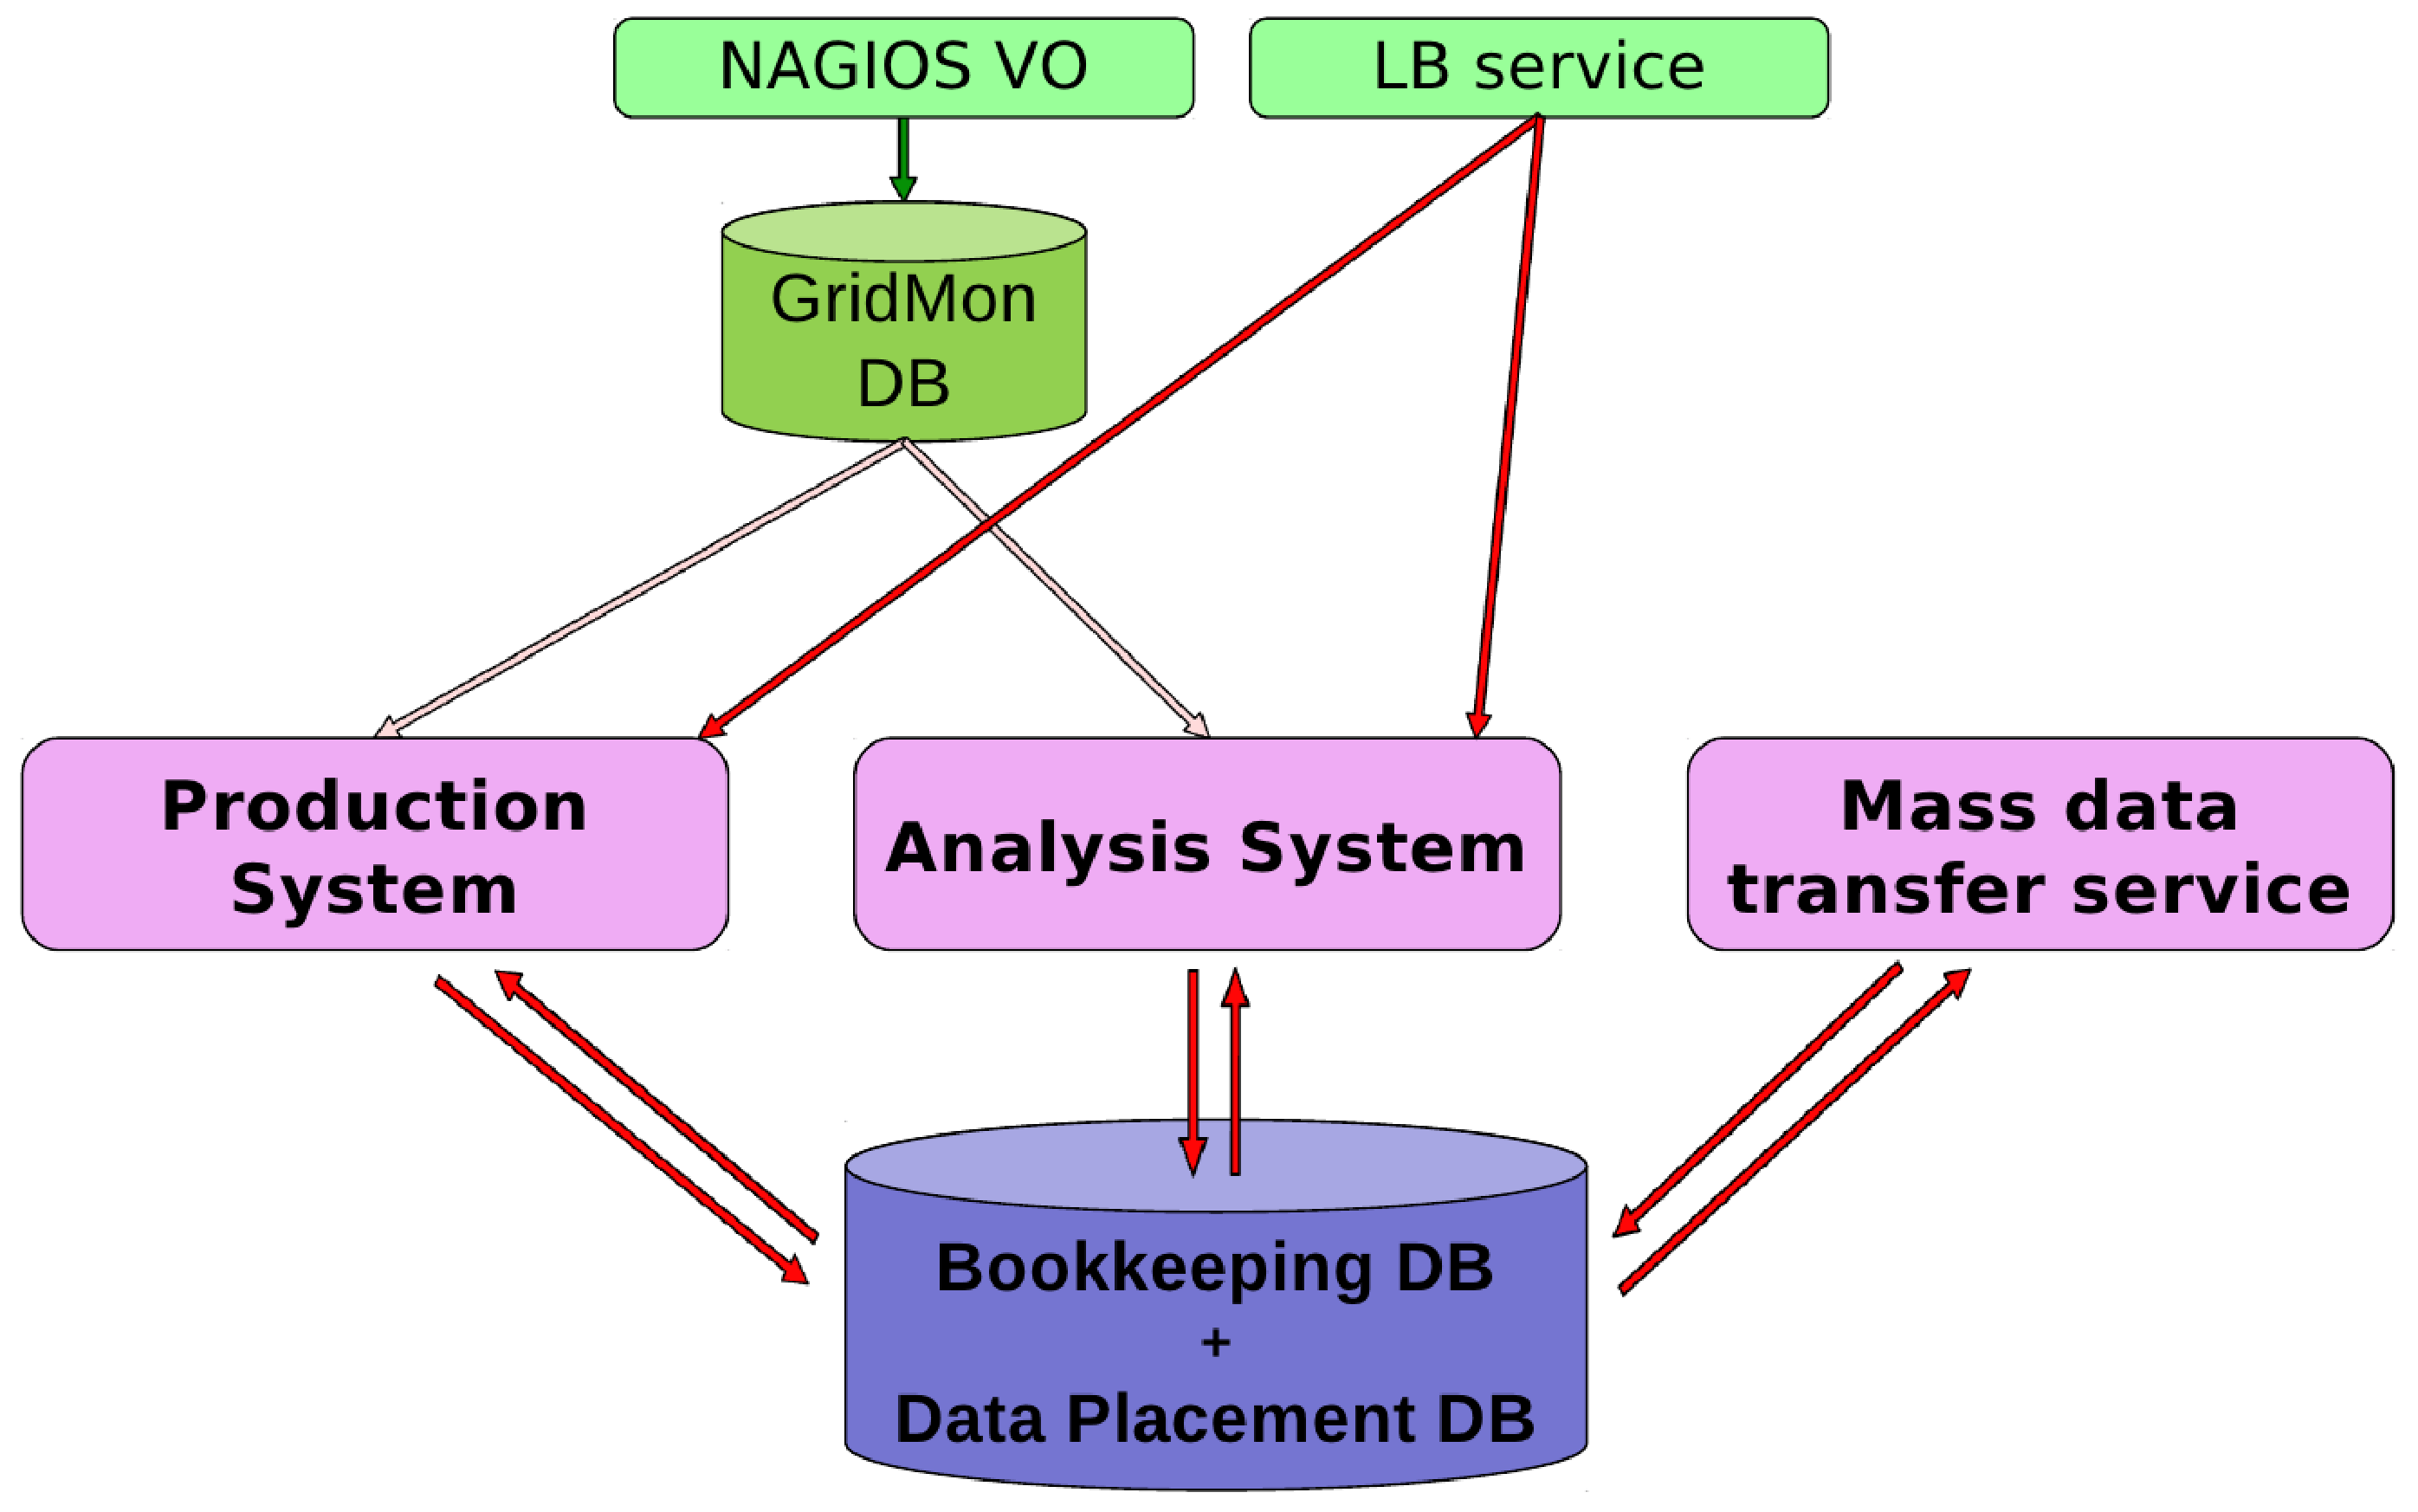
\includegraphics[width=26pc]{img/distributed_system_bird_eye.eps}\hspace{2pc}%
\caption{\label{fig:distributed_system_bird_eye_view}Distributed System bird's eye view.}
\end{figure}
 
\section{The Dirac extension} 
% Rafal
- extension structure description\\
- Dirac general purpose project short description + Dirac configuration\\
- service and systems description in detail\\
- web interface components description\\


\section{Bookkeeping DB integration}
% Milosz -> SQLAlchemy
% Luca, Christian -> SBK
- Software layer based on SQLAlchemy\\
-- advantages using SQLAlchemy: Object relational Mapping, clean code, fast\\
-- development, change of DB backend\\
- BK description, highlighting the general purpose characteristics\\
-- session, request, dataset concept\\


\begin{figure}[h]
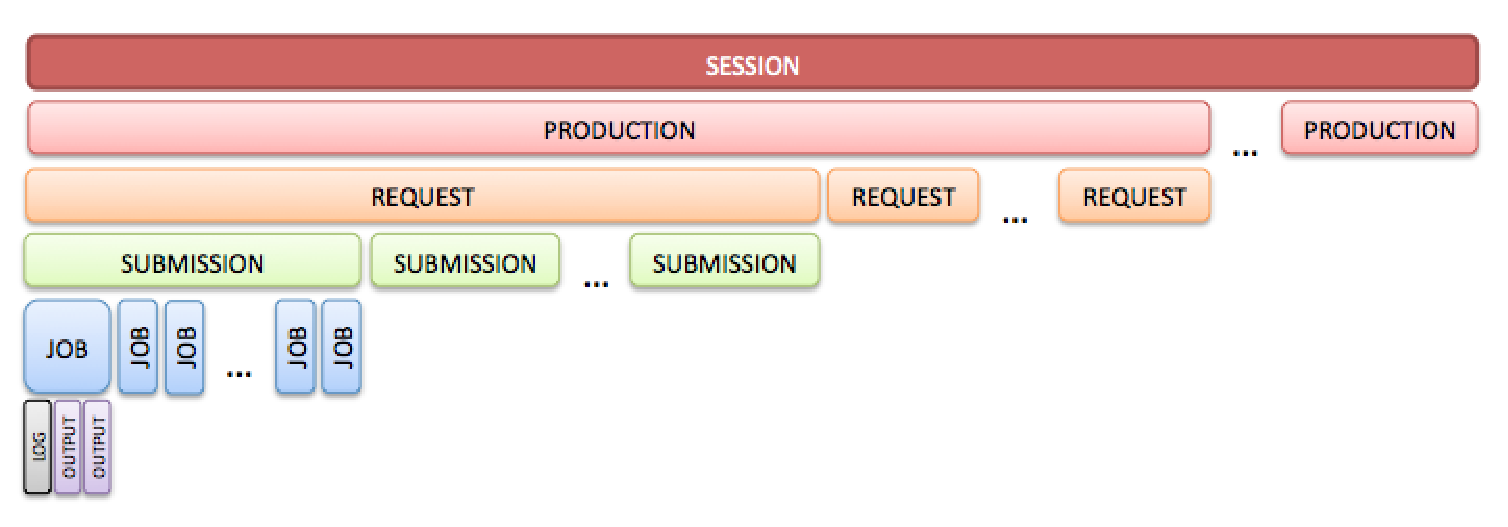
\includegraphics[width=26pc]{img/BK_entities.eps}\hspace{2pc}%
\caption{\label{fig:BK_entities}Entities in BookKeeping database.}
\end{figure}
 
\section{Job wrapper component}
% Bruno, Armando
- general workflow\\
- data management policy: stage-in and stage out strategies\\
 
\section{Simulation production use case: the SuperB experience}
% Bruno
- general description: workflow, Dirac portal design\\
- past experience: the webui project\\
-- Session definition interface --> DB dynamic build up\\

\begin{figure}[h]
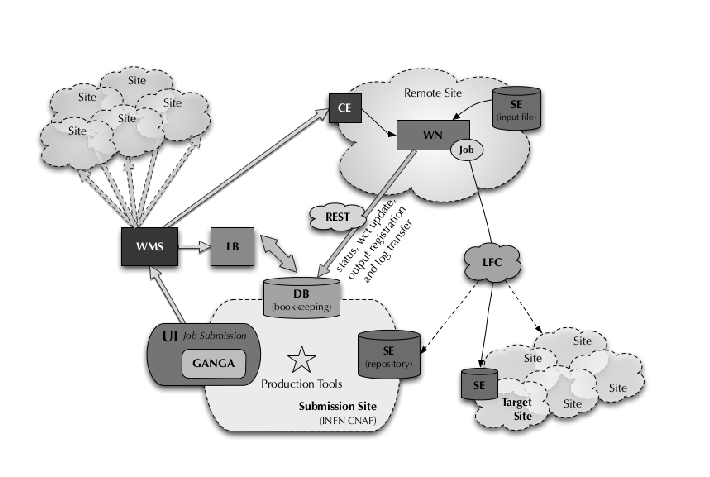
\includegraphics[width=26pc]{img/simulation_production_system_workflow.eps}\hspace{2pc}%
\caption{\label{fig:simulation_production_workflow}Simulation Production workflow.}
\end{figure}
 
\begin{figure}[h]
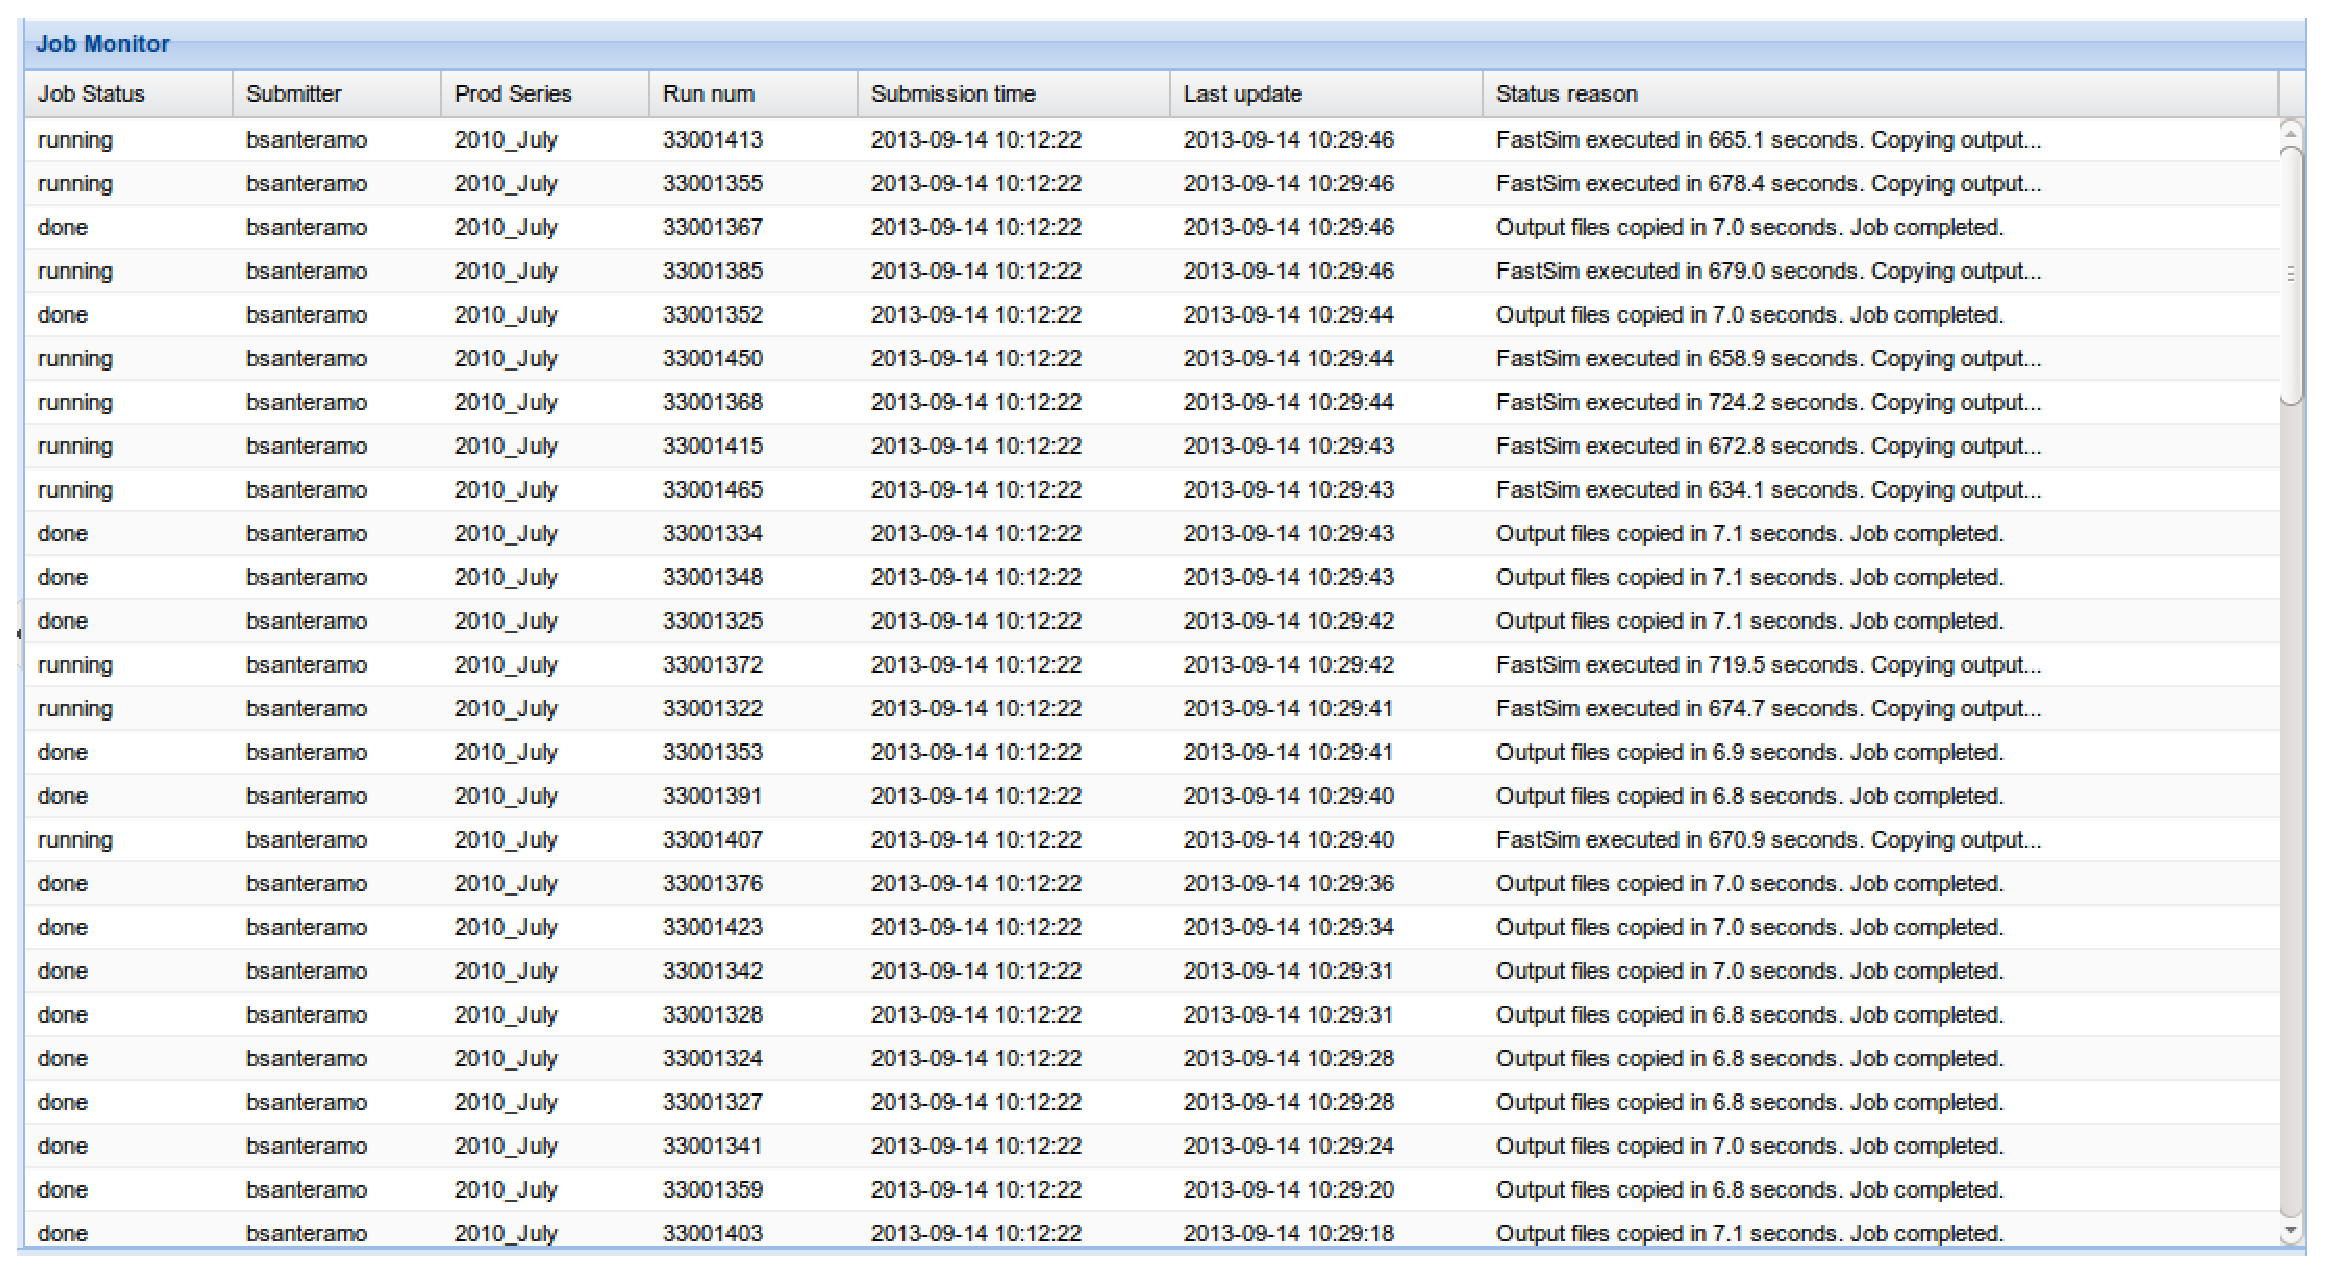
\includegraphics[width=26pc]{img/SuperBDIRAC_monitoring.eps}\hspace{2pc}%
\caption{\label{fig:superbdirac_monitoring}Monitoring job data from SBK in DIRAC.}
\end{figure}

\section{Functionality Test}
% Bruno
A functionality test was performed to demonstrate the capability of SuperBDIRAC to integrate the monitoring of a bookkeeping database in DIRAC webportal.
\subsection{Goal description}
DIRAC capabilities and performance as job management tool are well documented (insert some reference). Super$B$ distributed simulation stack (WebUI + SBK + Severus) was successfully used in 3 simulation campaigns (ask to Armando for confirmation and references).\\
Functionality Test goal is to demonstrate if SuperBDIRAC is capable of substitute WebUI as monitoring tool for job submission, showing data from a bookkeeping database. Test "Q-factor" is the exact correspondence of information as stored in SBK and displayed in SuperBDIRAC, like in WebUI monitoring page. Correct execution of simulation jobs is not important while the bookkeping information are properly managed.

\subsection{Testbed description}

\begin{figure}[h]
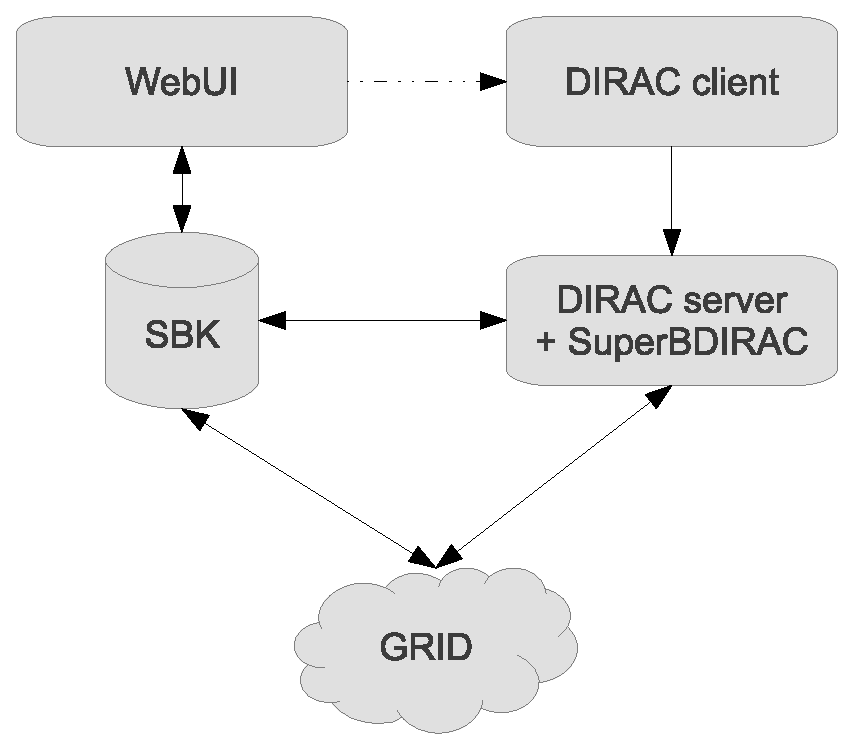
\includegraphics[width=14pc]{img/testbed.eps}\hspace{2pc}%
\begin{minipage}[b]{14pc}\caption{\label{label}Testbed schema.}
\end{minipage}
\end{figure}

At present time, not all WebUI functionalities are implemented in SUperBDIRAC, in particular "Submission" job for a given "Request".
The following procedure was followed to perform this test. FastSim job submission is created via WebUI interface. Once submission is created, a set of scripts and configuration files are created whose path is reported by WebUI interface: in particular the path of php submission script is taken to be be parsed. This php submission script, generated by WebUI, is made of an array with all relevant parameters and commands to UI in order to submit jobs in grid via standard glite commands.
Since WebUI is still linked with SBK, this portal could be used as well as monitoring portal, useful for a check-cross between info displayed in SBK, WebUI and SuperBDIRAC.\\

The php submission script is parsed by a python script (mc\_production.py), in particular the params array, in order to retrieve all needed paramenters to properly submit jobs: production series, session name, min and max runnumber, configuration files location, physical parameters, events to simulate. Once taken all these parameters, mc\_production.py uses DIRAC API to prepare and submit jobs via DIRAC client.

DIRAC server receive jobs from DIRAC client, than starts the normal workflow for job management in DIRAC: scheduling, pilot submission, payload retrieval and execution, stageout. Since DIRAC server is equipped with SuperBDIRAC, even bookkeeping monitoring is performed by this component.\\

In SBK the job submission insertion is performed by WebUI, while later info are updated by Severus script executed with every job submitted. Severus interact with SBK via REST interface, while WebUI and SuperBDIRAC have direct access to SBK since they are in the same LAN area (ask to Armando for confirmation).\\

Jobs were submitted via grid by DIRAC server. Submission was performed using WMS instead of using direct submission to CREAM CE.\\

Submission site was INFN-T1, which ensured CPU time to execute latest simulations related to Super$B$ once the experiment closure.

\subsection{Test description}

Every job simulated 3000 events: this value is set to have an execution time quite longer than 10 minutes.
Physical parameters are the same of other official productions.
3 main bunch submission of 400 jobs were performed at INFN-T1 to obtain a total of 1200 simulations.
Status in SBK were "prepared", "running" and "done".
In addition, 2 bunch submission of 10 jobs were performed, again at INFN-T1, to force some failure message in SBK and catch it even in SuperBDIRAC monitoring. First failure sample was obtained setting a not-existing site as destination for stageout: error was detected during preliminary check, so status in SBK were "prepared" and "failed". In second failure sample, jobs were submitted using a proxy without Role=ProductionManager, so error occurred in stageout phase: status in SBK were "prepared", "running" and "failed". In summary, 1220 jobs were submitted for test.\\

Since test goal, several screenshots of WebUI and SuperBDIRAC monitoring were saved, in addition to SBK data screenshots.

\subsection{Results and conclusions}

For each tests, all jobs were submitted at same time. Job execution depends on queue occupancy. Since we were interested in bookkeeping database status updates and not in measuring DIRAC performance in job execution, no dedicated CPU slots were asked for. While failing jobs were all executed simultaneously (10 dedicated CPU were always available for Super$B$ at INFN-T1), for 400 jobs tests simulation execution was spread on a greater time interval (see table \ref{tab:execution_time}).

\begin{table}[h]
\caption{
  \label{tab:execution_time}
  Execution time calculated as difference between Submission time and End Time in DIRAC scheduling system.
}
\begin{center}
\begin{tabular}{lrrr}
\br
test & mean time (sec) & min time (sec) & max time (sec)\\
\mr
good-1 & 2203,66 & 859,00 & 5048,00\\
good-2 & 1102,92 & 832,00 & 2597,00\\
good-3 & 1188,62 & 849,00 & 4716,00\\
failure-1 & 165,10 & 161,00 & 172,00\\
failure-2 & 901,50 & 874,00 & 935,00\\
\br
\end{tabular}
\end{center}
\end{table}

Mean and max time could be interesting for performance measurements, but for this functionality test min time must be considered since it's related to execution time of job ran once submitted. First 3 good test have similar min time, compatible with estimated 13 minutes for simulation. For failure test, in first case the low min time is due to forced error in preliminary check phase (jobs fail without executing simulation code), in second case jobs execute simulation code but fail trying stageout (due to wrong Role-based permission in writing INFN-T1 storage area), so min time is longer as expected.

\begin{table}[h]
\caption{\label{tab:status_update}Job status in SBK, WebUI and SuperBDIRAC.}
\begin{center}
\begin{tabular}{lrlrrrr}
\br
test & jobs & site & SBK status & WebUI status & SuperBDIRAC status & success rate\\
\mr
good-1 & 400 & INFN-T1 & 3 & 3 & 3 & 100\%\\
good-2 & 400 & INFN-T1 & 3 & 3 & 3 & 100\%\\
good-3 & 400 & INFN-T1 & 3 & 3 & 3 & 100\%\\
failure-1 & 10 & INFN-T1 & 2 & 2 & 2 & 100\%\\
failure-2 & 10 & INFN-T1 & 3 & 3 & 3 & 100\%\\
\br
\end{tabular}
\end{center}
\end{table}

BookKeeping database was properly updated for every job in every test. All status change were promptly displayed as well in SuperBDIRAC as in WebUI, without any appreciable delay between two portals. SQLAlchemy didn't introduced any appreciable delay or information loss, at least in this functionality test. 
Table \ref{tab:status_update} reports, for every test, how many status were saved in SBK and displayed in WebUI and SuperBDIRAC. Success rate was established as ratio between status saved in SBK and status displayed in SuperBDIRAC: its value was 100\% in all submissions.
SuperBDIRAC could be considered good enough to integrate in DIRAC the capability of monitoring jobs metadata from a bookkeeping database.

\section{Conclusions}

- We are offering a Dirac extended suite capable to satisfy the
needs on small and mid size VOs in terms of distributed
resource exploitation....

%% \begin{figure}
%% \begin{center}
%% \includegraphics[width=30pc]{schema.pdf}
%% \caption{Dirac suite design schema}
%% \label{fig:superb_sites}
%% \end{center}
%% \end{figure}


\section*{References}
%%%%%%%%%%%%%%%%%%%%%%%%%%%%%%%%%%%%%%%%%%%

\begin{thebibliography}{30}
%% \bibitem{superb}
%% The Super$B$ Collaboration, \emph{SuperB Progress Report, Detector},
%% \verb"http://arxiv.org/abs/1007.4241v1"

%% \bibitem{ref:miur}
%% \verb"http://www.istruzione.it/web/hub/home"

%% \bibitem{ref:babar}
%% Aubert B et al., 2002 {\it Nucl. Instr. Meth. Phys. Res.}, A 479, 1.

%% \bibitem{ref:belle}
%% The Belle Collaboration 2002 The Belle Detector, {\it Nucl. Instrum. Methods Phys. Res.}, Sect. A 479, 117.

%% \bibitem{atlas}
%% The ATLAS Collaboration, {\it ATLAS Detector and Physics Performance Technical Design
%% Report}, http://atlas.web.cern.ch/Atlas/GROUPS/PHYSICS/TDR/access.html.

%% \bibitem{cms}
%% The CMS Collaboration, {\it CMS Detector Technical Design Report}, http://cmsdoc.cern.ch/cms/cpt/tdr/.

%% \bibitem{ref:chep_dist}
%% Bianchi F, Brown D, Corvo M, Di Simone A, Fella A, Gianoli A, Luppi E, 
%% Morandin M, Paoloni E, Rama M, Tomassetti L 2010 {\it Computing for the Next
%% Generation Flavour Factories}, Proceeding of conference CHEP 2010, Computing for
%% High Energy Physics, Taipei, Taiwan, 18-22 October 2010

%% \bibitem{ref:fast_ieee}
%% Andreassen R et al 2010 {\it FastSim: fast simulation of the SuperB detector},
%% Proceeding of conference IEEE NSS-MIC 2010, Knoxville, TN, USA

%% \bibitem{ref:fast_sim}
%% Di Simone A, Gaponenko I, Manoni E, Perez A, Rama M, Roberts D, 
%% Rotondo M, Simi G, Sokoloff M, Suzuki A, Walsh J 2010 {\it FastSim: fast
%% simulation of the SuperB detector}, Proceeding of conference IEEE NSS-MIC
%% 2010,
%% Knoxville, TN, USA

%% %\bibitem{ref:chep_prod} 
%% %D. Brown, M. Corvo, A. Di Simone, A. Fella, E. Luppi, E. Paoloni, R. Stroili, L.
%% %Tomassetti, \emph{The Distributed Production System of the Super$B$ Project:
%% %Description and Results}. Proceeding of conference CHEP 2010, Computing for High
%% %Energy Physics, Taipei, Taiwan, 18-22 October 2010

%% \bibitem{ref:ieee_prod}
%% Brown D, Corvo M, Di Simone A, Fella A, Luppi E, Paoloni E, Stroili R and Tomassetti L 2010 {\it First Results from the SuperB Simulation Production System}. Proceeding of conference IEEE 2010, NSS-MIC 
%% 2010, Knoxville, TN, USA

%% \bibitem{ref:babar_cm}
%% Bozzi C, Adye T, Andreotti D, Antonioli E, Barlow R, Bense B, Boutigny D, Brew C A J, Colling D, Cowles R D, Elmer P, Feltresi E, Forti A, Grosdidier G, Hasan A,  Lacker H, Luppi E, Martyniak J, McNab A, Petzold A, Smith D A, Sundermann J E and Veronesi P 2003 {\it Using the Grid for the BaBar Experiment}, Nuclear Science Symposium Conference Record, 2003 IEEE, 1626 - 1629 Vol.3

%% %N. Geddes \emph{The BaBar Computing Model}. SLAC-PUB-9964, April 1994

%% \bibitem{egi} 
%% \verb"http://www.egi.eu"

%% \bibitem{osg} 
%% \verb"http://www.opensciencegrid.org"

%% \bibitem{dirac} 
%% \verb"http://diracgrid.org"

%% %\bibitem{ref:nordugrid} 
%% %\verb"http://www.norduGrid.org"

%% \bibitem{ref:westgrid} 
%% \verb"http://www.westgrid.ca"

%% \bibitem{ref:lcg-tdr} 
%% The LCG TDR Editorial Board 2005 {\it LHC Computing Grid}, Technical Design
%% Report LCG-TDR-001 CERN-LHCC-2005-024

%% \bibitem{ref:ganga}
%% \verb"http://ganga.web.cern.ch/ganga"

%% \bibitem{ref:wms}
%% \verb"http://glite.web.cern.ch/glite"

%% \bibitem{ref:voms}
%% \verb"http://hep-project-grid-scg.web.cern.ch/hep-project-grid-scg/voms.html"

%% \bibitem{ref:lfc}
%% \verb"https://twiki.cern.ch/twiki/bin/view/LCG/LfcAdminGuide"

%% \bibitem{lcg}
%% \verb"http://lcg.web.cern.ch/LCG"

%% \bibitem{ref:srm}
%% \verb"http://sdm.lbl.gov/srm-wg/doc/SRM.v2.2.html"

%% \bibitem{ref:storm}
%% Corso A et al. 2006 {\it StoRM, an SRM Implementation for LHC Analysis Farms
%% Computing in High Energy Physics} (CHEP 2006), Mumbai, India, Feb. 13-17

%% \bibitem{ref:dcache}
%% Fuhrmann P and Glzow V, dCache 2006 {\it Storage System for the Future}.
%% New York: Lecture Notes in Computer Science/Springer, vol. 4128, pp.
%% 1106-1113.

%% \bibitem{ref:dpm}
%% \verb"https://twiki.cern.ch/twiki/pub/LCG/DataManagementUsefulPresentations/chep 07\_poster_DPM.ppt"

%% \bibitem{ref:hadoop}
%% \verb"http://hadoop.apache.org/"

\bibitem{ref:superb_tdr}
Super$B$ Technical Design Report, \verb"http://arxiv.org/abs/1306.5655"

\bibitem{ref:rest}
Fielding R T 2000 {\it Architectural Styles and The Design of Network-based
Software Architectures }, PhD Thesis, University of California Irvine

\bibitem{ref:webui}
A.Fella, E.Luppi, L.Tomassetti \emph{A General Purpose Suite for Job Management, Bookkeeping and Grid Submission}. International Journal of Grid Computing \& Applications (IJGCA) Vol.2, No.2, June 2011. DOI: 10.5121/ijgca.2011.2202.

\end{thebibliography}


\end{document}


